\documentclass[12pt, a4paper, normaltoc, capchap, capsec, times]{abnt}

\usepackage[brazilian]{babel}
\usepackage[utf8]{inputenc}
\usepackage{wrapfig}
\usepackage{multirow}
\usepackage{amsthm}
\usepackage{amsfonts}
\usepackage{amsmath}
\usepackage[ruled,lined,portuguese]{algorithm2e}
\usepackage{graphicx}
\usepackage[config]{subfig}
\usepackage{abntcite}
\usepackage{uff}

\begin{document}

\looseness+1

\begin{resumo}
Essa monografia tem por objetivo implantar e avaliar a técnica de \emph{ranking reduzido a classificação binária} descrita no artigo \cite{langford08}. Tal técnica pertence à área de estudo chamada \emph{Learning to Rank} inserida na macroárea de Aprendizado de Máquina no campo de Inteligência Artificial. O problema emerge de situações reais como: ordenar documentos de acordo com uma busca e escolha de produtos a serem recomendados em um \emph{e-commerce}.
\end{resumo}

\begin{abstract}
This monograph has for goal to implement and evaluate a reduction from ranking to classification as proposed in \cite{langford08}. Such technique belongs to an area named Learning to Rank, inserted in Machine Learning branch in the field of Artificial Inteligence. The problem arises from real situations as: document ordering according to some query and selection of products to recommend in a e-commerce.
\end{abstract}

\chapter{Introdução}
\label{chap:introducao}
\begin{frame}
    Introdução
\end{frame}

\chapter{\emph{Ranking}: Noções Preliminares}
\label{chap:nocoes_preliminares}
Na área de \emph{aprendizado de máquina}, classificação é a tarefa de atribuir rótulos a cada elemento de um dado conjunto tendo como entrada pares elemento-rótulo. Comparativamente, \emph{ranking} é a tarefa de atribuir posições a cada elemento de um dado conjunto tendo como entrada pares elemento-rótulo, uma relação de ordem parcial entre os elementos, ou uma relação de ordem total entre os elementos \cite{tieyan09}.

Embora desempenhem tarefas diferentes com saídas diferentes, algoritmos de classificação e de \emph{ranking} podem compartilhar o mesmo tipo de entrada: pares elemento-rótulo. Isso é uma evidência de que se pode usar um algoritmo de classificação para compor um algoritmo de \emph{ranking}.

De fato, a técnica de \emph{ranking} descrita em \cite{langford08} propõe envolver  um algoritmo de classificação com etapas de pré-processamento e pós-processamento de forma que o produto final seja uma ordenação. Nesse estudo, essa técnica é chamada de \emph{ranking reduzido a classificação}.

\section{Introdução ao problema}

Dado um conjunto composto por elementos aos quais é possível atribuir um rótulo de valor $0$ ou $1$, deseja-se encontrar uma permutação dos elementos de maneira que os elementos que apresentem maior chance de receber o rótulo $0$ devem preceder os com maior chance de receber o rótulo $1$. Cada elemento é composto por um conjunto de características e a chance de um elemento receber o rótulo $0$ ou o rótulo $1$ deve ser calculada com base nessas características.

Substituindo-se a palavra rótulo pela palavra classe no enunciado acima, percebe-se que o problema de ordenação pode ser tratado como um problema de classificação. Mais especificamente, um problema de classificação binária, pois os valores de classe possíveis são $0$ e $1$.

Um algoritmo de aprendizado para classificação recebe como entrada um conjunto em que cada elemento possui uma classe assinalada e, partindo dessa entrada, deve aprender um classificador capaz de atribuir uma classe a novos elementos. A etapa em que o aprendizado ocorre é chamada de treinamento.

O treinamento de um classificador é um aprendizado supervisionado, pois cada elemento submetido à etapa de treinamento está vinculado à sua classe verdadeira. Dessa forma, pode-se medir a qualidade do classificador aprendido usando elementos com classes conhecidas, porém suprimindo-as quando os elementos forem submetidos a classificação.

O produto da classificação de um elemento é uma previsão do valor da classe à qual aquele elemento pertence. Sobre a previsão é possível obter uma quantidade de certeza, ou probabilidade, do elemento pertencer à classe prevista. Nesso caso, por se tratar de um problema de classificação binária, se a probabilidade de um elemento pertencer à classe $0$ é $p$, então a probabilidade dele pertencer à classe $1$ é $1 - p$.

Uma solução trivial para o problema de ordenação é utilizar a probabilidade das previsões de um classificador como uma relação de ordem no conjunto a ser ordenado. De posse da previsão das classes dos elementos de um dado conjunto, basta ordená-los de forma crescente em função da probabilidade de cada um pertencer à classe $0$; os mais prováveis ocupam o topo, os menos prováveis ocupam o fundo.

Segundo \cite{langford08}, esse método para ordenação dos elementos pode resultar em um erro teórico máximo muito alto, dependendo da performance do classificador. A técnica de \emph{ranking reduzido a classificação}, proposta no mesmo artigo, reduz o erro teórico máximo envolvendo o treinamento do classificador com uma etapa de pré-processamento e a avaliação com uma etapa de pós-processamento.

Na técnica de \emph{ranking reduzido a classificação}, o treinamento do classificador ocorre pelo algoritmo \emph{AUC-Train} após uma etapa inicial em que se aplica uma transformação nos exemplos da base de treinamento. Após o treinamento, a definição da ordem das instâncias na base de avaliação é feita pelo algoritmo \emph{tournament} --- torneio em português --- que usa as previsões do classificador treinado para tal.

\section{Definições}

Como dito anteriormente, o treinamento e avaliação de um classificador é um processo que manipula conjuntos compostos por elementos. Definições mais rigorosas são necessárias para a descrição da implementação da técnica de \emph{ranking reduzido a classificação} no capítulo \ref{chap:implantacao}. As definições abaixo foram feitas levando-se em consideração o funcionamento da ferramenta WEKA e os requisitos necessários para se modelar a solução de \emph{ranking reduzido a classificação} exposta em \cite{langford08}.

\begin{itemize}
    \item Uma base $S$ é um conjunto de instâncias com cardinalidade $n$.
    \[S = \{i_1, ..., i_n\} \qquad |S| = n\]

    \item Uma instância $I$ é uma tupla $\langle x, y \rangle$ na qual $x$ é um vetor de atributos com cardinalidade $m$ e $y$ é a classe da instância e pode valer $0$ ou $1$.
    \[I = \langle x, y \rangle \qquad x = \{a_1, ..., a_m\} \qquad y \in \{0, 1\}\]
\end{itemize}

Pode-se acessar os atributos de uma instância $I$ através de $x_I$ e a classe através de $y_I$. Pode-se, também, concatenar os vetores de atributos de duas instâncias $I$ e $I'$ através da operação $(x_I, x_{I'})$.

Não será necessária a definição do conceito de atributo. Uma vez que os atributos são manipulados pelo classificador e o funcionamento dos classificadores nas soluções aqui propostas é uma caixa preta, os atributos são transparentes para os propósitos desse trabalho.

A tabela \ref{tab:weather} apresenta um exemplo de base extraído do livro \cite{wekabook}. Essa base indica se há condições para a prática de um esporte de acordo com medições meteorológicas. Um exemplo dessa base apresenta um conjunto de medições meteorológicas e, de acordo com essas medições, a classe do exemplo pode ser \emph{sim} ou \emph{não}.

\begin{table}[h!]
    \centering
    \begin{tabular}{ccccc}
        \hline
        panorama & temperatura & umidade & ventoso & adequado para jogo \\
        \hline
        ensolarado & quente & alta & falso & não \\
        ensolarado & quente & alta & verdadeiro & não \\
        nublado & quente & alta & falso & sim \\
        chuvoso & branda & alta & falso & sim \\
        chuvoso & frio & normal & falso & sim \\
        chuvoso & frio & normal & verdadeiro & não \\
        nublado & frio & normal & verdadeiro & sim \\
        ensolarado & branda & alta & falso & não \\
        ensolarado & frio & normal & falso & sim \\
        chuvoso & branda & normal & falso & sim \\
        ensolarado & branda & normal & verdadeiro & sim \\
        nublado & branda & alta & verdadeiro & sim \\
        nublado & quente & normal & falso & sim \\
        chuvoso & branda & alta & verdadeiro & não \\
        \hline
    \end{tabular}

    \caption{Base de dados de tempo. \label{tab:weather}}
\end{table}


A primeira linha nomeia os quatro atributos da base e a classe (adequado para jogo), as linhas seguintes representam as instâncias da base. Nota-se que a classe recebe valores \emph{sim} e \emph{não}, apesar de serem valores diferentes de $0$ e $1$, como dito na definição, ainda se trata de uma base com classe binária.

Escrevendo a primeira instância da base na notação definida acima, tem-se: ((ensolarado, quente, alta, falso), não). O primeiro elemento da tupla é o vetor de atributos e o segundo elemento é a classe da instância.


\section{Medidas de desempenho}

Geralmente, a medida de eficiência mais utilizada para classificação é a acurácia: uma razão entre o número de instâncias corretamente classificadas sobre o número total de instâncias no conjunto de avaliação.

O erro decorrente de uma classificação afeta a acurácia de maneira linear. Como, para ordenações, a quantidade de acertos não é tão relevante quanto a posição das instâncias ordenadas, propõe-se outro tipo de medida para avaliação do \emph{ranking} aprendido.

Uma medida comum de avaliação para algoritmos de \emph{ranking} é a área sobre a curva \emph{ROC (Receiver Operating Characteristic)}, comumente chamada de \emph{AUC (Area Under the Curve)}.

A perda, $1 - AUC$, associada a essa medida é calculada pelo número de instâncias, normalizado pela quantidade de $0$s vezes a quantidade de $1$s, que necessitam ser trocadas para um \emph{ranking} perfeito.

Uma ordenação é perfeita quando todas as instâncias com classe $0$ precedem as com classe $1$, nesse caso a perda na \emph{AUC} é $0$. No pior caso, em que todos os $1$s precedem os $0$s, a perda na \emph{AUC} é $1$.

Comparativamente, um erro de classificação pode ter maior influência na medida \emph{AUC} que na acurácia afetando consideravelmente um \emph{ranking}, mas não a classificação. A causa disso é a \emph{AUC} considerar a relação entre as instâncias ordenadas, enquanto a acurácia considera apenas erros e acertos pontualmente. A seguir, ilustramos, através de um exemplo, uma relação entre essas medidas que comprova o intuído sobre erros na classificação.

\begin{table}[h!]
    \centering
    \begin{tabular}{cccccc}
        \hline
        panorama & temperatura & umidade & ventoso & classe & previsão \\
        \hline
        ensolarado & quente & alta & falso & não & sim \\
        nublado & quente & alta & falso & sim & sim \\
        chuvoso & branda & alta & falso & sim & sim \\
        chuvoso & frio & normal & falso & sim & sim \\
        nublado & frio & normal & verdadeiro & sim & sim \\
        ensolarado & frio & normal & falso & sim & sim \\
        chuvoso & branda & normal & falso & sim & sim \\
        ensolarado & branda & normal & verdadeiro & sim & sim \\
        nublado & branda & alta & verdadeiro & sim & sim \\
        nublado & quente & normal & falso & sim & sim \\
        ensolarado & quente & alta & verdadeiro & não & não \\
        chuvoso & frio & normal & verdadeiro & não & não \\
        ensolarado & branda & alta & falso & não & não \\
        chuvoso & branda & alta & verdadeiro & não & não \\
        \hline
    \end{tabular}

    \caption{Exemplo de \emph{ranking} e classificação na base weather.\label{tab:exemplo}}
\end{table}

Na tabela \ref{tab:exemplo}, temos quatorze instâncias ordenadas em um \emph{ranking} com os atributos, as classes e as previsões dadas por um classificador. Podemos perceber que o classificador errou apenas a classe da primeira instância. Calculando a acurácia, temos treze acertos em quatorze possíveis, o que equivale a aproximadamente $93\%$ de acerto.

Calculando a perda da AUC considerando como base a classe \emph{sim}, a primeira instância precisa retroceder nove posições para uma ordenação perfeita, normalizando pelo número de \emph{não's} vezes o número de \emph{sim's}, temos $(1 - AUC) = 9 \div (5 * 9) = 0,2$, logo a AUC vale $80\%$. Esse exemplo comprova que a AUC pode sofrer um impacto maior devido a erros de classificação se comparada à acurácia.

De acordo com \cite{langford08}, se um classificador gera um erro de ordem $\alpha$ na acurácia, ao ordenar uma base a partir das probabilidades das previsões desse classificador, o erro teórico máximo na AUC será de $\alpha \cdot n$, onde $n$ é a cardinalidade da base avaliada. Enquanto para o mesmo classificador, a técnica de \emph{ranking reduzido a classificação} apresenta um erro teórico máximo de $\alpha \cdot 2$.

O erro na AUC se intensifica a medida que o desbalanceamento de classes do conjunto usado no treinamento aumenta, pois quanto mais desbalanceadas as classes, mais provável que o classificador resultante seja tendencioso para a classe majoritária.

\chapter{\emph{Ranking}: Implantação}
\label{chap:implantacao}
\begin{frame}
    \frametitle{AUC-Train}

    \begin{algorithm}[H]
        $S' = \{\langle (x_1, x_2), 1(y_1 < y_2) \rangle \; : \; (x_1, y_1), (x_2, y_2) \in S \; and \; y_1 \neq y_2$\;
        \Return{$c = A(S')$}

        \caption{AUC-Train}
    \end{algorithm}

    \begin{block}{Decomposição}
        \begin{enumerate}
            \item Particionar a base de treinamento em duas bases $S_0$ e $S_1$; $S_0$ possui as instâncias de classe $0$ e $S_1$ possui as instâncias de classe $1$;
            \item Combinar as partições $S_0$ e $S_1$ de forma que a base de treinamento $S'$ possua todos os pares entre instâncias de classe $1$ e de classe $0$;
            \item Aplicar um algoritmo de aprendizagem $A$ à base $S'$ obtendo um classificador $c$ como saída.
        \end{enumerate}
    \end{block}
\end{frame}

\begin{frame}
    \frametitle{AUC-Train: Particionamento}

    \begin{function}[H]
        $S_0, S_1 \gets \emptyset$\;

        \ParaTodo{$i \in S$}{
            \eSe{$i(C) = 0$}{
                $S_0 \gets S_0 \cup \{ i \}$\;
            }{
                $S_1 \gets S_1 \cup \{ i \}$\;
            }
        }

        \Retorna{$S_0, S_1$}

        \caption{particionar($S$)}
    \end{function}

    \begin{block}{Complexidade}
        \begin{itemize}
            \item $O(n)$
        \end{itemize}
    \end{block}
\end{frame}

\begin{frame}
    \frametitle{AUC-Train: Combinação}

    \begin{function}[H]
        $S_C \gets \emptyset$\;

        \ParaTodo{$\alpha \in S_{\alpha}$}{
            \ParaTodo{$\beta \in S_{\beta}$}{
                $S_C \gets S_C \cup \{ mesclar(\alpha, \beta) \}$\;
            }
        }

        \Retorna{$S_C$}

        \caption{combinar($S_{\alpha}, S_{\beta}$)}
    \end{function}

    \begin{function}[H]
        \Retorna{$\langle \alpha(A) || \beta(A), 1 \cdot (\alpha(C), \beta(C)) \rangle$}

        \caption{mesclar($\alpha, \beta$)}
    \end{function}

    \begin{block}{Complexidade}
        \begin{itemize}
            \item Melhor caso: $O(n)$
            \item Caso médio e pior caso: $O(n^2)$
        \end{itemize}
    \end{block}
\end{frame}

\begin{frame}
    \frametitle{AUC-Train: Otimizações}

    \begin{block}{Desvantagem}
        O custo computacional adicionados pelas etapa de particionamento e principalmente pela etapa de combinação é alto.
    \end{block}

    \begin{block}{Sugestões de Otimização}
        \begin{itemize}
            \item Votação
            \item Amostragem
        \end{itemize}
    \end{block}

    Há uma complementaridade entre as duas estratégias escolhidas para otimização do algoritmo AUC-Train. Enquanto uma preza por melhorar o tempo de execução, o outra preza por dar maior segurança na classificação.
\end{frame}

\begin{frame}
    \frametitle{AUC-Train: Otimização - Amostragem}

    \begin{function}[H]
        $S \gets \emptyset$\;

        \ParaTodo{$\alpha \in S_{\alpha}$}{
            \ParaTodo{$\beta \in Ss_{\beta} \; tal\; que\; Ss_{\beta} \subseteq S_{\beta} \wedge |Ss_{\beta}| = p$}{
                $S \gets S \cup \{ mesclar(\alpha, \beta) \}$\;
            }
        }

        \Retorna{$S$}

        \caption{amostragem($S_{\alpha}, S_{\beta}, p$)}
    \end{function}
\end{frame}

\begin{frame}
    \frametitle{Algoritmo de Treinamento}

    \begin{algorithm}[H]
        $C \gets \emptyset$\;
        $S_0, S_1 \gets particionar(S)$;

        \Se{$i = 1$ e $p = todas$}{
            $S' \gets combinar(S_0, S_1, mesclar)$\;
            $S' \gets combinar(S_1, S_0, mesclar)$\;
            $C \gets \{ A(S') \}$\;
        }
        \SenaoSe{$i > 1$ e $0 < p \leq min(|S_0|, |S_1|)$}{
            \Para{$i \gets 1; i \to n$}{
                $S' \gets amostragem(S_0, S_1, p, mesclar)$\;
                $S' \gets S' \cup amostragem(S_1, S_0, p, mesclar)$\;
                $C \gets C \cup \{ A(S') \}$\;
            }
        }

        \Retorna{$C$}

        \caption{Treinamento}
    \end{algorithm}
\end{frame}

\begin{frame}
    \frametitle{Tournament}

    \begin{algorithm}[H]
        For $x \in U$, let $deg(x) = |\{x':c(x, x') = 1, x' \in U\}|$\;
        Sort U in descending order of deg(x), breaking ties arbitrarily

        \caption{Tournament}
    \end{algorithm}

    \begin{block}{Decomposição}
        \begin{enumerate}
            \item Obter a pontuação para todas as instâncias na base $B$;
            \item Ordenar as instâncias na base $B$.
        \end{enumerate}
    \end{block}
\end{frame}

\begin{frame}
    \frametitle{Tournament: Efeito Colateral - Votação}

    \begin{function}[H]
        $classe \gets 0$\;
        $zero \gets 0$\;

        \ParaTodo{$c \in C$}{
            \eSe{$c(i) = 0$}{
                $zero \gets zero + 1$\;
            }{
                $zero \gets zero - 1$\;
            }
        }

        \Se{$zero < 0$}{
            $classe \gets 1$\;
        }

        \Retorna{$classe$}

        \caption{votacao(C, i)}
    \end{function}
\end{frame}

\begin{frame}
    \frametitle{Algoritmo de Ordenação}

    \begin{algorithm}[H]
        \ParaTodo{$\alpha \in B$}{
            \ParaTodo{$\beta \in B \wedge \beta \neq \alpha$}{
                $i \gets \langle \alpha(A) || \beta(A) \rangle$\;
                $classe \gets votacao(C, i)$

                \eSe{$classe = 1$}{
                    $pontuacao[\alpha] \gets pontuacao[\alpha] + 1$
                }{
                    $pontuacao[\beta] \gets pontuacao[\beta] + 1$
                }
            }
        }

        ordenar $B$ com base em $pontuacao$

        \caption{Ordenação}
    \end{algorithm}

    \begin{block}{Complexidade}
        \begin{itemize}
            \item $O(n^2)$ chamadas à função votacao + $O(f_{sort}(n))$;
        \end{itemize}
    \end{block}
\end{frame}

\chapter{Avaliação do \emph{Ranking}}
\label{chap:avaliacao}
De acordo com o artigo \cite{langford08} e como dito no capítulo \ref{chap:nocoes_preliminares}, um classificador que apresente um erro $\alpha$ na acurácia, pode apresentar um erro teórico máximo de $\alpha \cdot n$, onde $n$ é a cardinalidade da base a ser ordenada. A técnica de \emph{ranking reduzido a classificação} diminui esse limite para $\alpha * 2$ usando o mesmo classificador com erro $\alpha$ na acurácia.

Quanto maior o desbalanceamento entre as classes da base a ser ordenada, maior a chance de intensificação do erro na ordenação. Partindo desse princípio, foi montada uma estratégia de testes com cinco bases de dados com diferentes níveis de desbalanceamento. Tais bases podem ser encontradas no repositório da University of California, Irvine (UCI)\footnote{http://archive.ics.uci.edu/ml/}.

\section{Características das bases}

As bases usadas foram as seguintes: Breast Cancer; Statlog (Vehicle Silhouettes), chamada de Vehicle; Hepatitis; Glass Identification, chamada de Glass e Yeast. Como o algoritmo proposto em {{langford}} tem um custo computacional alto, $O(n^2)$ para treinamento e $O(n^2)$ para gerar o ranking; isso aliado ao baixo controle sobre o ambiente de execução culminou na escolha de bases pequenas para avaliação do experimento.

As bases Vehicle, Glass e Yeast tratam, originalmente, de problemas multiclasse. A essas bases foram aplicadas transformações, descritas em \cite{guo04}, a fim de torná-las problemas de classe binária. Para as bases Vehicle e Glass, foram unidas todas as classes, exceto a minoritária, em uma nova classe. Para a base Yeast, apenas as classes de valor 'CYT' ou 'POX' foram consideradas.

Cada base utilizada apresenta diferenças em: desbalanceamento entre as classes, número de atributos, número de instâncias, entre outros. A tabela \ref{tbl:caracteristicas} mostra um resumo sobre as características das bases.

\begin{table}[h]

    \begin{tabular}{c c c c c c c}
        \hline
        \multirow{2}{*}{Bases} & \multicolumn{2}{c}{Atributos} & \multirow{2}{*}{Instâncias} & \multicolumn{3}{c}{Classe} \\ \cline{2-3} \cline{5-7}
        & {\small Contínuos} & {\small Discretos} & & {\small Minoritária} & {\small Majoritária} & {\small Distribuição}\\
        \hline
        breast-cancer & 0 & 9 & 286 & 85 & 201 & 30\% - 70\%\\
        vehicle & 18 & 0  & 846 & 199 & 647 & 23\% - 77\%\\
        hepatitis & 6 & 13  & 155 & 32 & 123 & 20\% - 80\%\\
        glass & 9 & 0  & 214 & 29 & 185 & 13\% - 87\%\\
        yeast & 8 & 0  & 483 & 20 & 463 & 4\% - 96\%\\
        \hline
    \end{tabular}

    \caption{Dados sobre as bases usadas para \emph{ranking}. \label{tbl:caracteristicas}}
\end{table}

\section{Execução e Avaliação do Algoritmo}
\label{sec:avaliacao}

Foram escolhidos quatro classificadores base para avaliar o algoritmo: J48, Naïve Bayes, Logistic e SMO. O motivo da escolha desses classificadores é o reconhecimento de tais como padrões em suas famílias, J48 para árvores de decisão (implanta a árvore de decisão C4.5), Naïve Bayes para estatísticos, Logistic (implanta curva logística) e SMO (implanta Support Vector Machine) para classificadores baseados em funções.

Para cada classificador base houve quatro baterias de execução com diferentes configurações:

\begin{enumerate}

    \item Somente o classificador;
    \item O classificador como base para a técnica de \emph{ranking reduzido a classificação} original;
    \item O classificador como base para o algoritmo de ranking com configurações de 1 par por instância e variando o número de classificadores na votação entre 1 e 20;
    \item O classificador como base para o algoritmo de ranking com configurações de 1 classificador na votação e variando o número de pares por instância entre 1 e 20.

\end{enumerate}

Nas três baterias que envolveram o algoritmo de \emph{ranking}, o método de ordenação usado para gerar o resultado final foi o \emph{torneio}, como explicado no artigo {{langford}}. Em todas as baterias foi executada uma validação cruzada com 10 partições e os resultados apresentados nas tabelas é a média das \emph{AUCs} obtidas para cada partição.

Para as tabelas de número \ref{j48_results_table}, \ref{nb_results_table}, \ref{logistic_results_table} e \ref{smo_results_table}; o símbolo \textbf{*} significa ranking aplicado com 1 par por instância e 10 classificadores na votação. O símbolo \textbf{**} significa ranking aplicado com 10 pares por instância e 1 classificador na votação.

\clearpage
\pagebreak

\subsection{Desempenho para \emph{C4.5} (trees.J48)}


\begin{table}[h!]
    \begin{tabular}{ c c c c c }
        \hline
    
        \multirow{2}{*}{Bases} & \multirow{2}{*}{J48} & \multicolumn{3}{c}{J48 acrescido de} \\ \cline{3-5}
        & & {\small Ranking Original} & {\small Ranking*} & {\small  Ranking**} \\

        \hline
        
        breast-cancer & {\small \textbf{0,62806 (0,01005)}} & {\small 0,46784 (0,03049)} & {\small 0,51289 (0,01950)} & {\small 0,45055 (0,02984)} \\
        vehicle & {\small 0,93725 (0,00056)} & {\small 0,91389 (0,00624)} & {\small \textbf{0.98072 (0.00017)}} & {\small 0,95670 (0,00071)} \\
        hepatitis & {\small 0,69655 (0,04084)} & {\small 0,67112 (0,03127)} & {\small \textbf{0,74322 (0,03925)}} & {\small 0,72179 (0,04571)} \\
        glass & {\small \textbf{0,90322 (0,01578)}} & {\small 0,83772 (0,03524)} & {\small 0,89016 (0,02934)} & {\small 0,88860 (0,02668)} \\
        yeast & {\small 0,48918 (0,00021)} & {\small \textbf{0,95009 (0,01453)}} & {\small 0,78550 (0,03630)} & {\small 0.84806 (0.01924)} \\
    
        \hline
    \end{tabular}
    
    \caption{Desempenho para árvore de decisão C4.5}
    \label{j48_results_table}
\end{table}

\begin{figure}[h!]
    \centering
    \subfloat[Breast cancer]{
        \label{fig:breast-cancer_j48}
        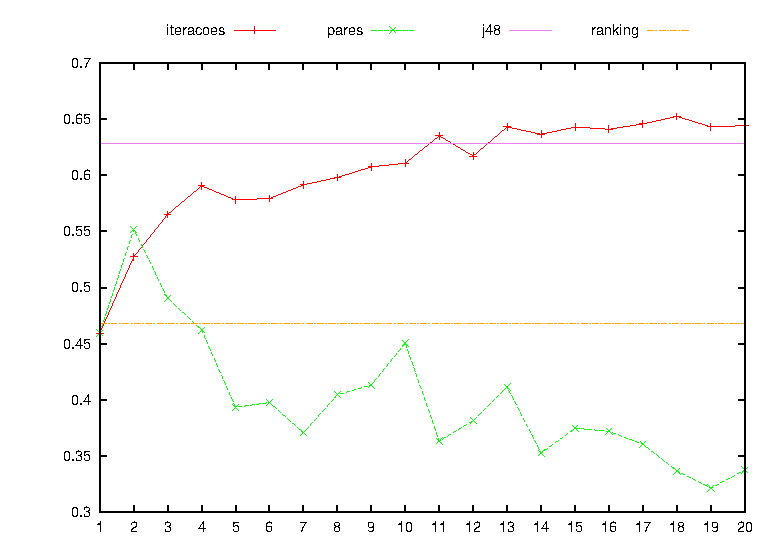
\includegraphics[width=0.42\textwidth]{img/breast-cancer_j48.eps}
    }
    \subfloat[Glass]{
        \label{fig:glass_j48}
        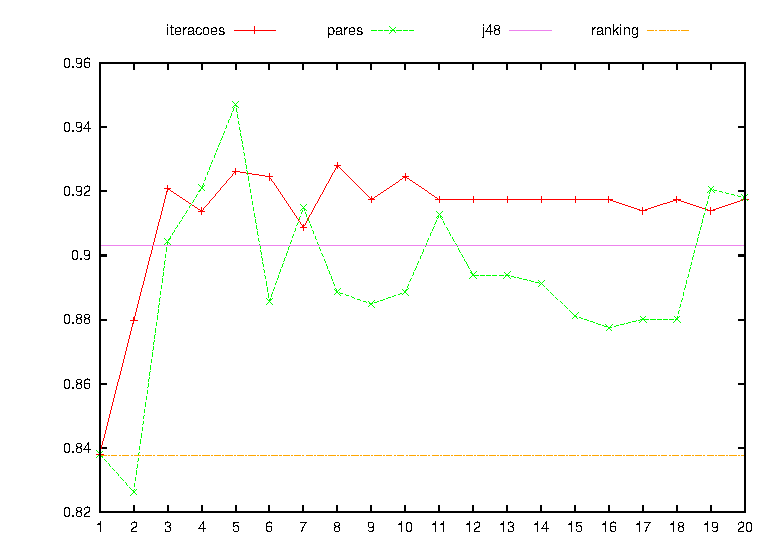
\includegraphics[width=0.42\textwidth]{img/glass_j48.eps}
    }

    \subfloat[Hepatitis]{
        \label{fig:hepatitis_j48}
        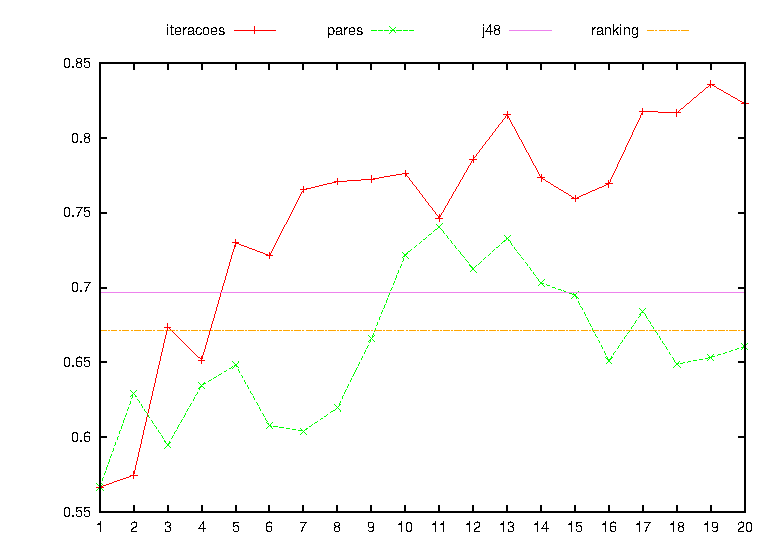
\includegraphics[width=0.42\textwidth]{img/hepatitis_j48.eps}
    }    
    \subfloat[Vehicle]{
        \label{fig:vehicle_j48}
        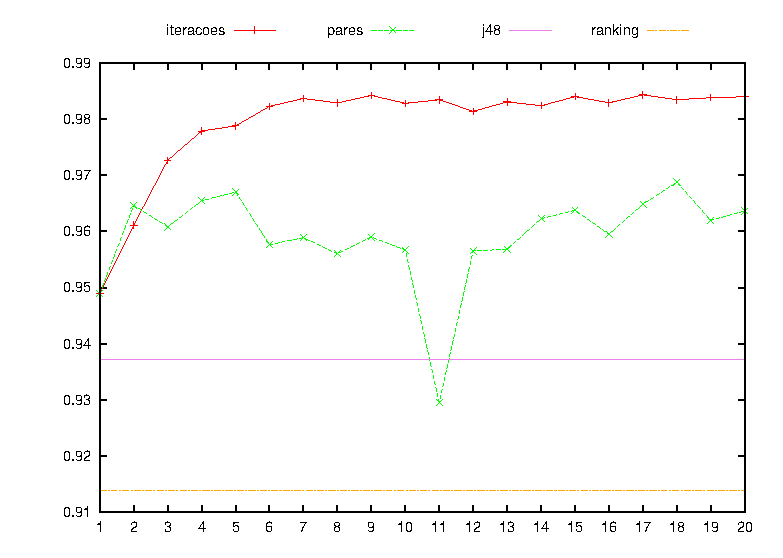
\includegraphics[width=0.42\textwidth]{img/vehicle_j48.eps}
    }

    \subfloat[Yeast]{
        \label{fig:yeast_j48}
        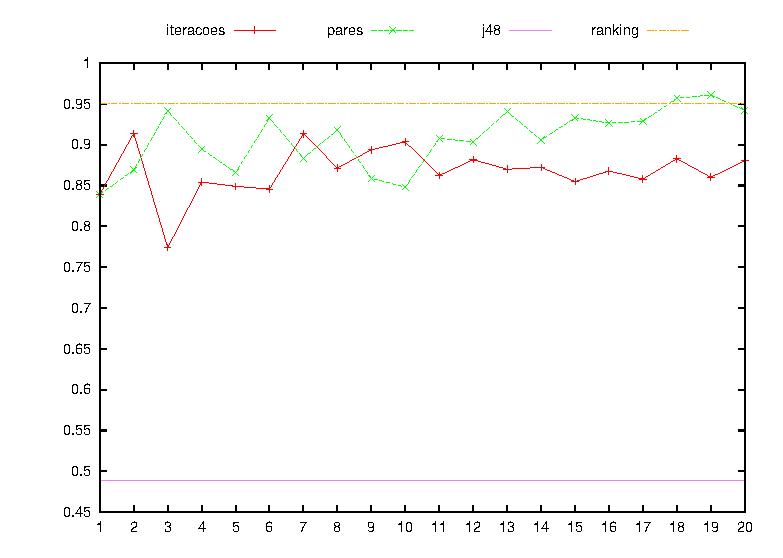
\includegraphics[width=0.42\textwidth]{img/yeast_j48.eps}
    }

    \caption{Gráficos de desempenho para árvore de decisão C4.5}
\end{figure}

\clearpage
\pagebreak


\subsection{Desempenho para \emph{Naïve Bayes} (bayes.NaiveBayes)}

\begin{table}[h!]
    \begin{tabular}{ c c c c c }
        \hline

        \multirow{2}{*}{Bases} & \multirow{2}{*}{Naïve Bayes} & \multicolumn{3}{c}{Naïve Bayes acrescido de} \\ \cline{3-5}
        & & {\small Ranking Original} & {\small Ranking*} & {\small  Ranking**} \\
    
        \hline
        
        breast-cancer & {\small \textbf{0,71543 (0,01899)}} & {\small 0,20857 (0,00620)} & {\small 0,04976 (0,00445)} & {\small 0,04532 (0,00426)} \\
        vehicle & {\small \textbf{0,80898 (0,00468)}} & {\small 0,24323 (0,01559)} & {\small 0,00310 (0,00004)} & {\small 0,12514 (0,01546)} \\
        hepatitis & {\small \textbf{0,85919 (0,01190)}} & {\small 0,22489 (0,05188)} & {\small 0,06052 (0,00265)} & {\small 0.06608 (0,00101)} \\
        glass & {\small \textbf{0,94084 (0,01099)}} & {\small 0,17271 (0,02416)} & {\small 0,02222 (0,00151)} & {\small 0,02476 (0,00132)} \\
        yeast & {\small 0,82863 (0.06355)} & {\small 0,84269 (0,03505)} & {\small \textbf{1,00000 (0,00000)}} & {\small \textbf{1,00000 (0,00000)}} \\
    
        \hline
    \end{tabular}
    
    \caption{Desempenho para Naïve Bayes}
    \label{nb_results_table}
\end{table}

\begin{figure}[h!]
    \centering
    \subfloat[Breast cancer]{
        \label{fig:breast-cancer_naive-bayes}
        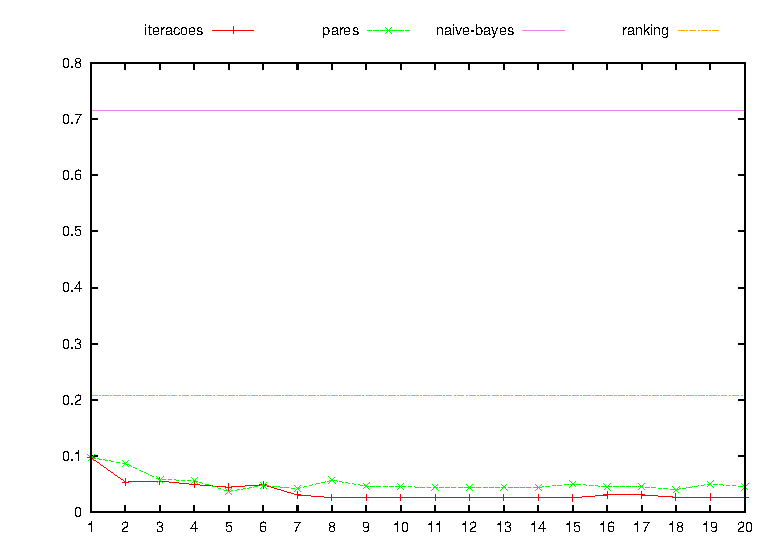
\includegraphics[width=0.42\textwidth]{img/breast-cancer_naive-bayes.eps}
    }
    \subfloat[Glass]{
        \label{fig:glass_naive-bayes}
        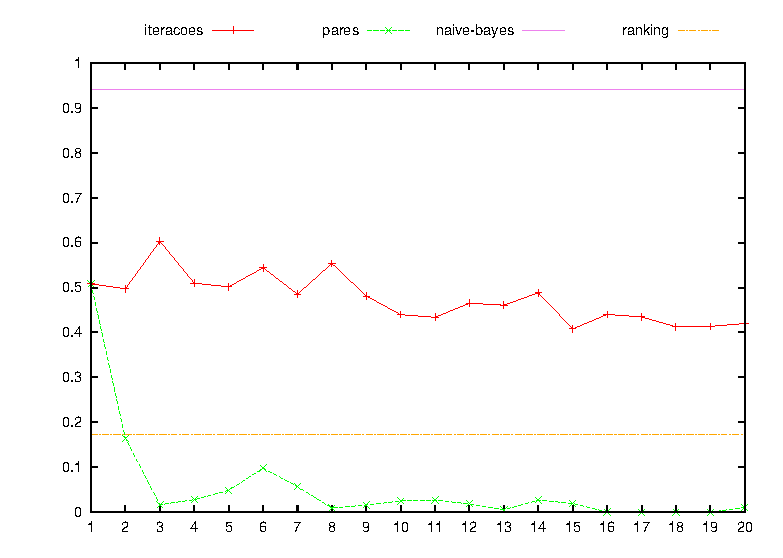
\includegraphics[width=0.42\textwidth]{img/glass_naive-bayes.eps}
    }

    \subfloat[Hepatitis]{
        \label{fig:hepatitis_naive-bayes}
        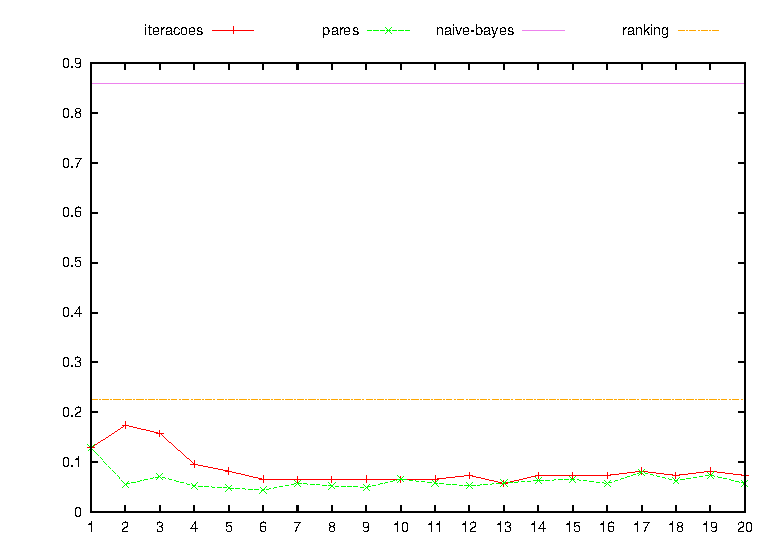
\includegraphics[width=0.42\textwidth]{img/hepatitis_naive-bayes.eps}
    }    
    \subfloat[Vehicle]{
        \label{fig:vehicle_naive-bayes}
        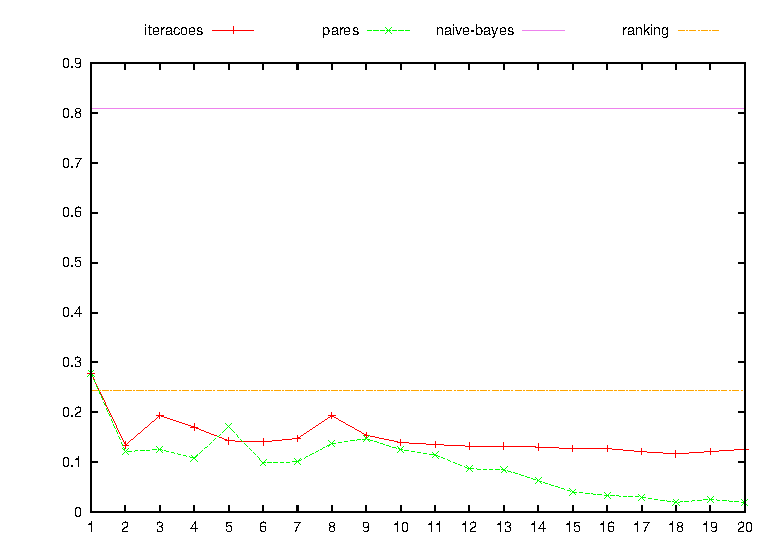
\includegraphics[width=0.42\textwidth]{img/vehicle_naive-bayes.eps}
    }

    \subfloat[Yeast]{
        \label{fig:yeast_naive-bayes}
        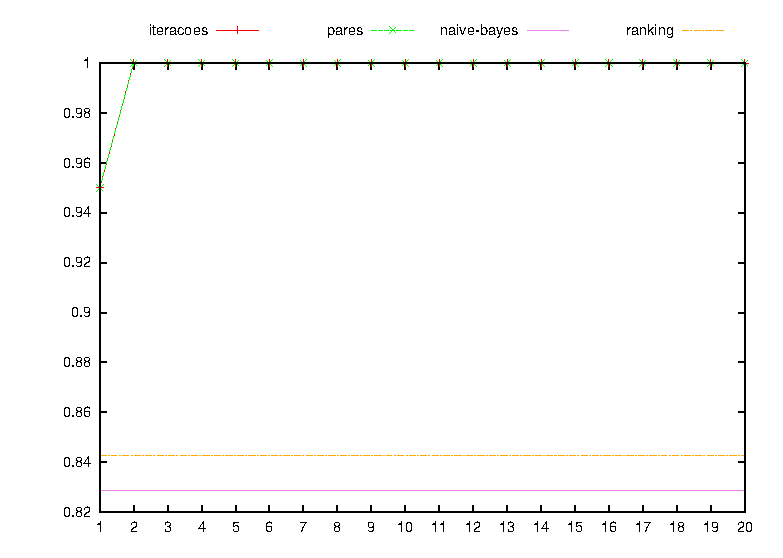
\includegraphics[width=0.42\textwidth]{img/yeast_naive-bayes.eps}
    }

    \caption{Gráficos de desempenho para Naïve Bayes}
\end{figure}

\clearpage
\pagebreak


\subsection{Desempenho para a \emph{Curva Logística} (functions.Logistic)}

\begin{table}[h!]
    \begin{tabular}{ c c c c c }
        \hline

        \multirow{2}{*}{Bases} & \multirow{2}{*}{Logistic} & \multicolumn{3}{c}{Logistic acrescido de} \\ \cline{3-5}
        & & {\small Ranking Original} & {\small Ranking*} & {\small  Ranking**} \\
        
        \hline
        
        breast-cancer & {\small 0,66625 (0,02322)} & {\small \textbf{0,66740 (0,02364)}} & {\small 0,65784 (0,02143)} & {\small 0,65132 (0,02219)} \\
        vehicle & {\small 0,99358 (0,00003)} & {\small \textbf{0,99420 (0,00003)}} & {\small 0,99358 (0,00003)} & {\small 0,99234 (0,00002)} \\
        hepatitis & {\small \textbf{0,80924 (0,02598)}} & {\small 0,79882 (0,02432)} & {\small 0,75064 (0,04278)} & {\small 0,74557 (0,05075)} \\
        glass & {\small 0,95965 (0,00308)} & {\small \textbf{0,97037 (0,00192)}} & {\small 0,96101 (0,00484)} & {\small 0,95536 (0,00384)} \\
        yeast & 0{\small ,85805 (0,04115)} & {\small 0,83453 (0,04931)} & {\small \textbf{0,87414 (0,03463)}} & {\small 0,85691 (0,03997)} \\
    
        \hline
    \end{tabular}
    
    \caption{Desempenho para Logistic}
    \label{logistic_results_table}
\end{table}

\begin{figure}[h!]
    \centering
    \subfloat[Breast cancer]{
        \label{fig:breast-cancer_logistic}
        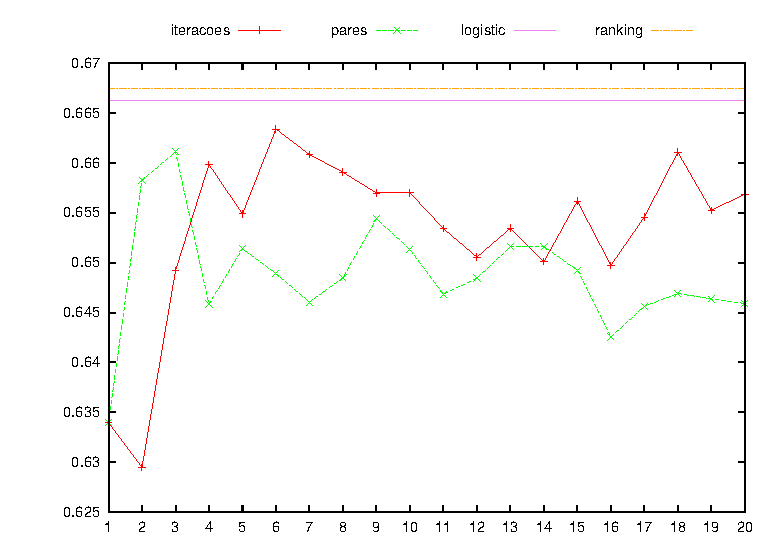
\includegraphics[width=0.42\textwidth]{img/breast-cancer_logistic.eps}
    }
    \subfloat[Glass]{
        \label{fig:glass_logistic}
        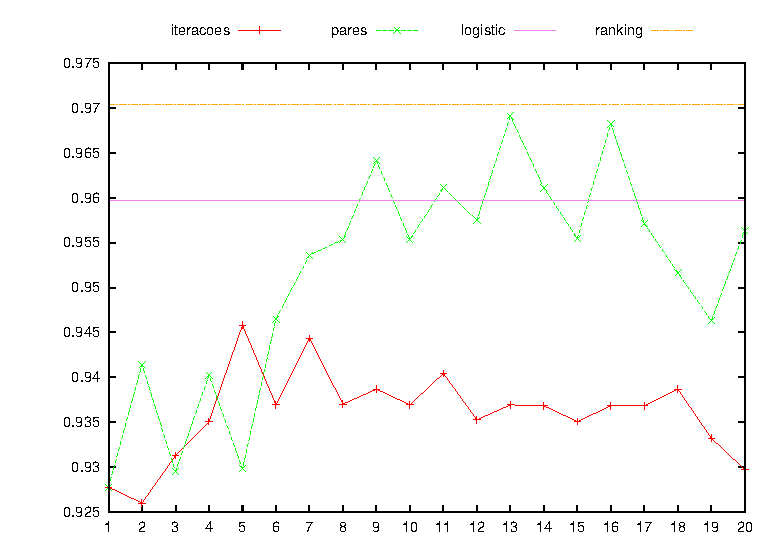
\includegraphics[width=0.42\textwidth]{img/glass_logistic.eps}
    }

    \subfloat[Hepatitis]{
        \label{fig:hepatitis_logistic}
        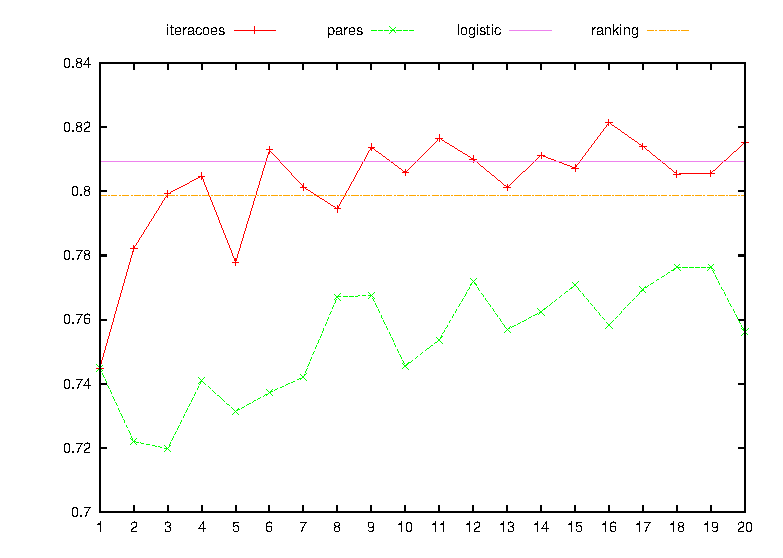
\includegraphics[width=0.42\textwidth]{img/hepatitis_logistic.eps}
    }    
    \subfloat[Vehicle]{
        \label{fig:vehicle_logistic}
        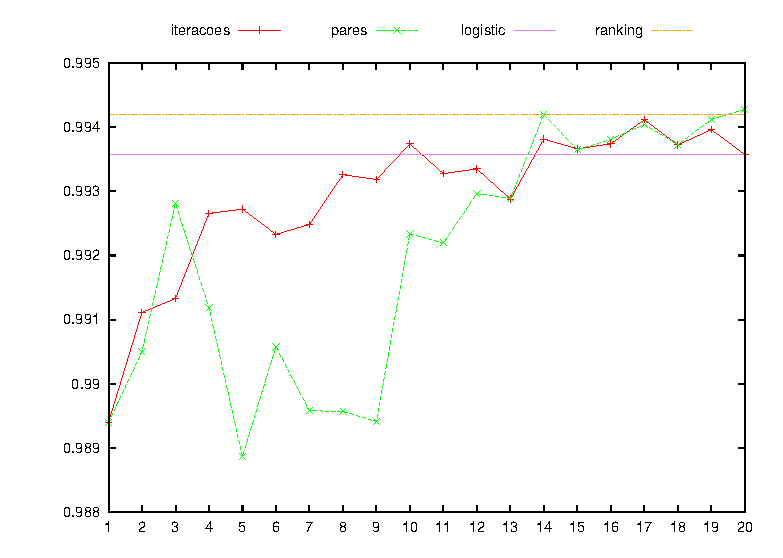
\includegraphics[width=0.42\textwidth]{img/vehicle_logistic.eps}
    }

    \subfloat[Yeast]{
        \label{fig:yeast_logistic}
        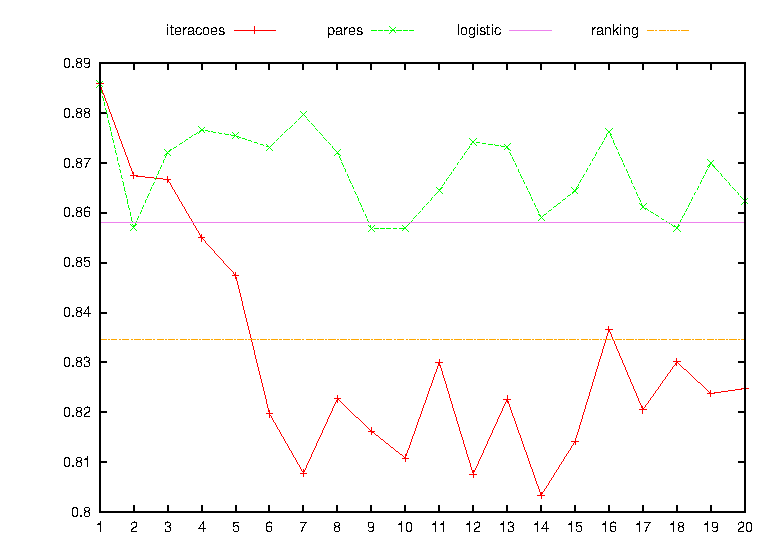
\includegraphics[width=0.42\textwidth]{img/yeast_logistic.eps}
    }

    \caption{Gráficos de desempenho para Curva Logística}
\end{figure}

\clearpage
\pagebreak


\subsection{Desempenho para \emph{Support Vector Machine} (functions.SMO)}

\begin{table}[h!]
    \begin{tabular}{ c c c c c }
        \hline

        \multirow{2}{*}{Bases} & \multirow{2}{*}{SMO} & \multicolumn{3}{c}{SMO acrescido de} \\ \cline{3-5}
        & & {\small Ranking Original} & {\small Ranking*} & {\small  Ranking**} \\
        
        \hline
        
        breast-cancer & {\small 0,59272 (0,00696)} & {\small \textbf{0,66670 (0,02294)}} & {\small 0,65832 (0,02119)} & {\small 0,65563 (0,02003)} \\
        vehicle & {\small 0,94434 (0,00169)} & {\small \textbf{0,99651 (0,00001)}} & {\small 0,99396 (0,00002)} & {\small 0,99380 (0,00002)} \\
        hepatitis & {\small 0,75128 (0,01618)} & {\small \textbf{0,81522 (0,01914)}} & {\small 0,80759 (0,01899)} & {\small 0,78189 (0,02640)} \\
        glass & {\small 0,89181 (0,00679)} & {\small \textbf{0,95712 (0,00175)}} & {\small 0,93402 (0,00610)} & {\small 0,93752 (0,00537)} \\
        yeast & {\small 0,77391 (0,04799)} & {\small 0,83555 (0,04831)} & {\small \textbf{0,99891 (0,00001)}} & {\small \textbf{0,99891 (0,00001)}} \\
    
        \hline
    \end{tabular}
    
    \caption{Desempenho para Support Vector Machine}
    \label{smo_results_table}
\end{table}

\begin{figure}[h!]
    \centering
    \subfloat[Breast cancer]{
        \label{fig:breast-cancer_smo}
        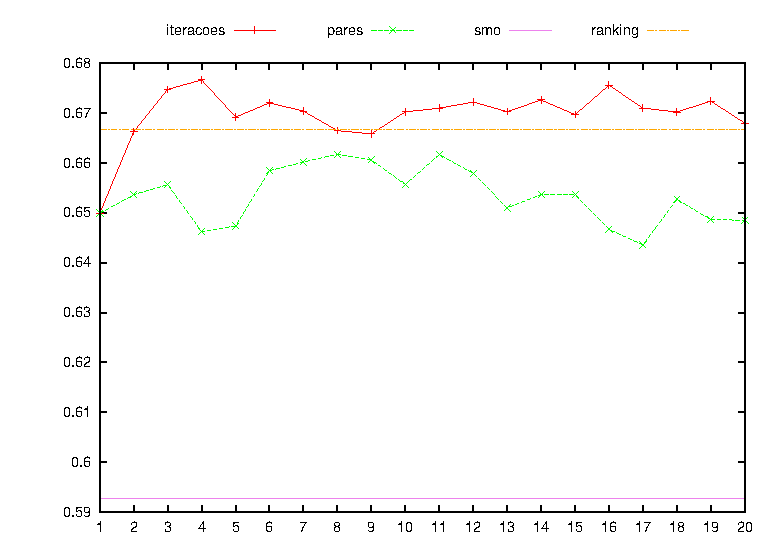
\includegraphics[width=0.42\textwidth]{img/breast-cancer_smo.eps}
    }
    \subfloat[Glass]{
        \label{fig:glass_smo}
        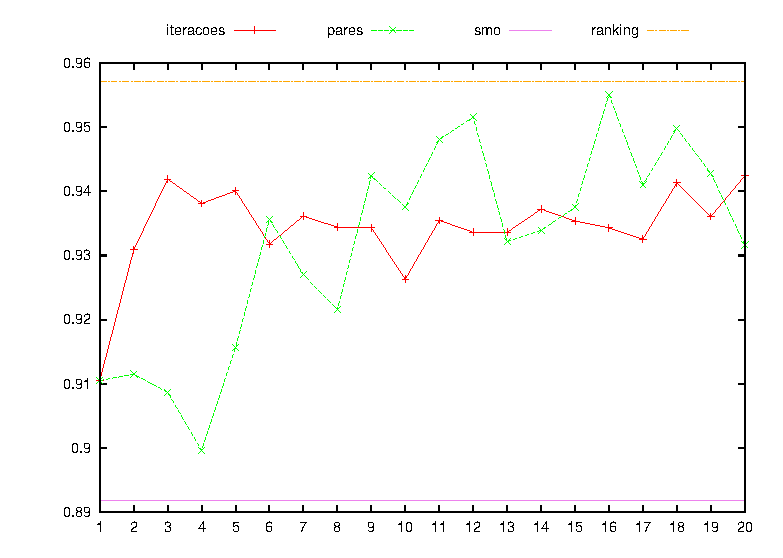
\includegraphics[width=0.42\textwidth]{img/glass_smo.eps}
    }

    \subfloat[Hepatitis]{
        \label{fig:hepatitis_smo}
        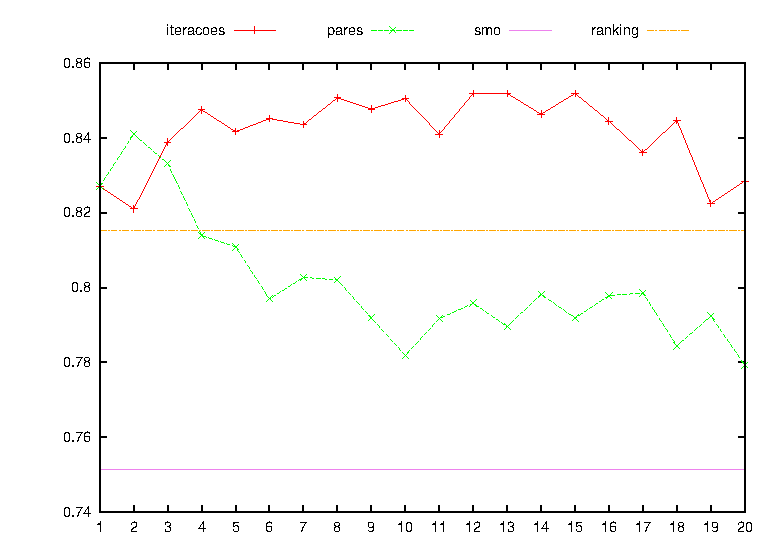
\includegraphics[width=0.42\textwidth]{img/hepatitis_smo.eps}
    }    
    \subfloat[Vehicle]{
        \label{fig:vehicle_smo}
        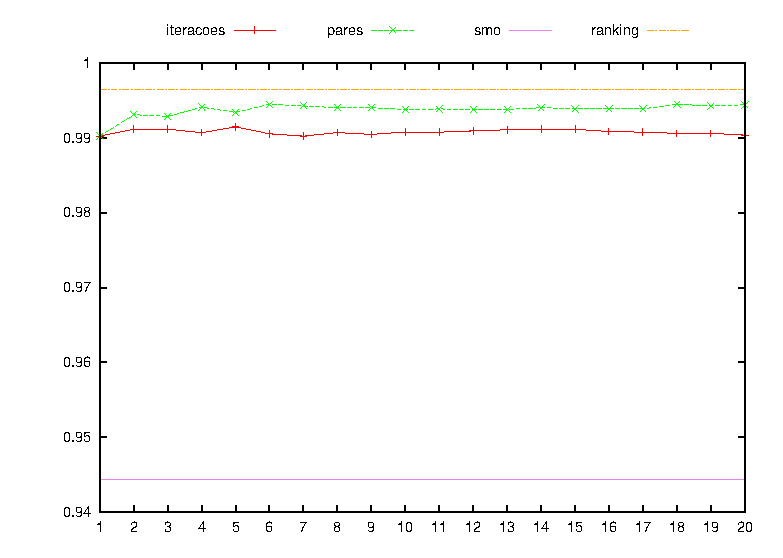
\includegraphics[width=0.42\textwidth]{img/vehicle_smo.eps}
    }

    \subfloat[Yeast]{
        \label{fig:yeast_smo}
        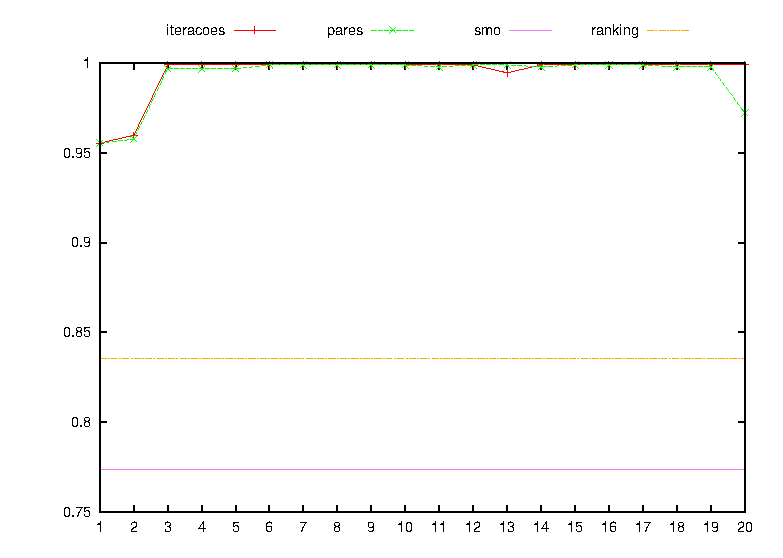
\includegraphics[width=0.42\textwidth]{img/yeast_smo.eps}
    }

    \caption{Gráficos de desempenho para Support Vector Machine}
\end{figure}

\chapter{Conclusão}
\label{chap:conclusao}
A primeira conclusão que pode ser tirada é que o algoritmo testado aqui tem uma performance muito baixa no que diz respeito a tempo computacional, tanto para treinamento, quanto para avaliação. As estratégias para melhoria no tempo de treinamento como uso de votação e de um número reduzido de pares por instância ajudaram nesse aspecto e criaram resultados por vezes superiores ao algoritmo original e ao classificador base.

Os esforços para otimizar o tempo na etapa de avaliação consistiram em implantar um algoritmo baseado no algoritmo \emph{Quicksort}, que teria tempo de execução médio $n\cdot\log{n}$, um avanço comparado ao tempo de execução médio do torneio que é $n^2$. Embora esta estratégia tenha sido completamente implantada, não houve nenhum experimento que a utilizasse.

O classificador Naïve Bayes teve um desempenho incomum quando combinado com o algortimo de \emph{Ranking}. Esse classificador gerou resultados muito abaixo do esperado para todas as bases testadas, exceto para a base \emph{yeast}.

Pode-se reparar que, para a base \emph{glass}, os resultados começam a melhorar em relação aos obtidos para as bases \emph{breast-cancer}, \emph{vehicle} e \emph{hepatitis}. Já para a base \emph{yeast}, o Naïve Bayes aliado ao algoritmo de \emph{Ranking} teve uma performance perfeita acertando quase todos as ordenações. Esse comportamento bipolar não foi elucidado nesse estudo.

Comparando as estratégias implantandas para acelerar a etapa de treinamento de forma isolada, pode-se chegar a seguinte conclusão: o aumento do número de classificadores na votação cria resultados mais com menor varição na AUC que o aumento de pares por instância no treinamento.

Olhando as curvas geradas para cada uma dessas estratégias nos gráficos do capítulo {{AVALIACAO}}, percebe-se que a tendência para a estratégia de aumento de classificadores na votação é, na maioria dos casos, crescente. Enquanto a tendência para a estratégia de aumento do número de pares por instância não pode ser definida com clareza em alguns casos.

O artigo [\cite{langford08}] mostra que um classificador que produza um erro $r$ na classificação pode produzir um erro teórico máximo de $n \cdot r$, onde $n$ é o número de exemplos a serem ordenados, na ordenação. Mostra também que o \emph{Ranking} gera produz um erro teórico máximo de $2 \cdot n$.

Não foi possível verificar a validade dessa prova teórica. Na maioria dos casos, a ordenação derivada apenas do classificador teve erro inferior ao erro na ordenação via algoritmo \emph{Ranking}.

\bibliography{monograph}

\end{document}
